%% LaTeX-Beamer template for KIT design
%% by Erik Burger, Christian Hammer
%% title picture by Klaus Krogmann
%%
%% version 2.1
%%
%% mostly compatible to KIT corporate design v2.0
%% http://intranet.kit.edu/gestaltungsrichtlinien.php
%%
%% Problems, bugs and comments to
%% burger@kit.edu

\documentclass[18pt]{beamer}
%% SLIDE FORMAT
\usepackage[utf8]{inputenc}
\usepackage{enumitem}
% use 'beamerthemekit' for standard 4:3 ratio
% for widescreen slides (16:9), use 'beamerthemekitwide'

%\usepackage{templates/beamerthemekit}
\usepackage{wrapfig}
\usepackage{hyperref}
\usepackage{algpseudocode}
\usepackage{graphicx}
\usepackage{epstopdf}

\epstopdfDeclareGraphicsRule{.gif}{png}{.png}{convert gif:#1 png:\OutputFile}
\AppendGraphicsExtensions{.gif}

 \newcommand{\real}{\mathbb{R}}
 \newcommand{\nat}{\mathbb{N}}
 \newcommand{\Oh}{\mathcal{O}}
 \newcommand{\oh}{\mathrm{o}}
 \newcommand{\SP}{\mathrm{SP}}

% \usepackage{templates/beamerthemekitwide}

%\usepackage{epigraph}

% for quotes

\AtBeginSection[] % Do nothing for \section*
{
\begin{frame}<beamer>
\frametitle{Gliederung}
\tableofcontents[currentsection]
\end{frame}
}


\usepackage{biolinum}

\usepackage{pgfplots}
\usepackage{filecontents}

\begin{filecontents}{data4.dat}
X	Y
22.5	2
20.5	2
16	2
12.5	1
6.5	2
\end{filecontents}


%% TikZ INTEGRATION

% use these packages for PCM symbols and UML classes
% \usepackage{templates/tikzkit}
% \usepackage{templates/tikzuml}

% the presentation starts here

\title[Algo I Tut]{5. Algorithmen Tutorium I}
\subtitle{Sortieralgorithmen - Intensiv}
\author[Zangerle]{Konstantin Zangerle}

\institute{Institut für Theoretische Informatik}

\usepackage{listings}
\usepackage{color}

\definecolor{mygreen}{rgb}{0,0.6,0}
\definecolor{mygray}{rgb}{0.5,0.5,0.5}
\definecolor{mymauve}{rgb}{0.58,0,0.82}

\lstset{ %
  backgroundcolor=\color{white},   % choose the background color
  basicstyle=\footnotesize,        % size of fonts used for the code
  breaklines=true,                 % automatic line breaking only at whitespace
  captionpos=b,                    % sets the caption-position to bottom
  commentstyle=\color{mygreen},    % comment style
  escapeinside={\%*}{*)},          % if you want to add LaTeX within your code
  keywordstyle=\color{blue},       % keyword style
  stringstyle=\color{mymauve},     % string literal style
}

% Bibliography

\begin{document}
\pgfplotstableread{data4.dat}{\blattIV}
% change the following line to "ngerman" for German style date and logos
%\selectlanguage{ngerman}

%title page
\begin{frame}
\titlepage
\end{frame}

%table of contents
\begin{frame}{Gliederung}
 \tableofcontents
\end{frame}


\section{Besprechung der Übungsaufgaben}
\begin{frame}{Übungblatt 3}
Häufige Fehler
\begin{itemize}
 \item Aufgabe 1) nur für n Zweierpotenz.
 \item Aufgabe 3) Geometrische Reihe für i = 0 
\end{itemize}
  \begin{tikzpicture}[scale=0.5]
 \begin{axis}[scaled x ticks={real:23}]
  \addplot table {\blattIV};
 \end{axis}
\end{tikzpicture}
\end{frame}


\begin{frame}{Bälle und Urnen}
 \begin{tabular}{lll}
  --- 				&	mit Zurücklegen 	& ohne Zurücklegen 	\\
 mit Beachtung d. Reihenfolge  	& 	$n^k$			& $\frac{n!}{(n-k)!}$	\\
 ohne Beachtung d .Reihenfolge 	& 	$\binom{n+k-1}{n-1}$	& $\binom{n}{k}$
 \end{tabular}

\end{frame}

\section{Sortieralgorithmen}
\begin{frame}[fragile]{Übersicht Sortieralgorithmen}
 \begin{itemize}
  \item Mergesort
  \item Insertionsort
  \item Selectionsort
  \item Quicksort
  \item Heapsort
  \item \verb|http://www.sorting-algorithms.com/|
 \end{itemize}

\end{frame}

\subsection{Mergesort}
\begin{frame}{Mergesort}
 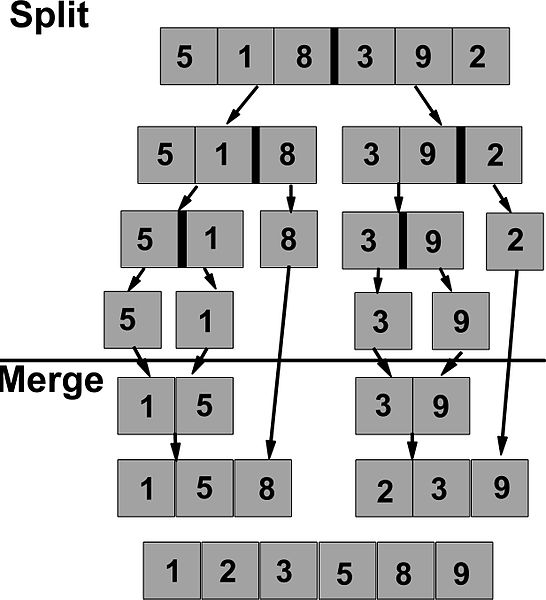
\includegraphics{MergeSort}
\end{frame}

\subsection{Insertionsort}
\begin{frame}{Insertionsort}
 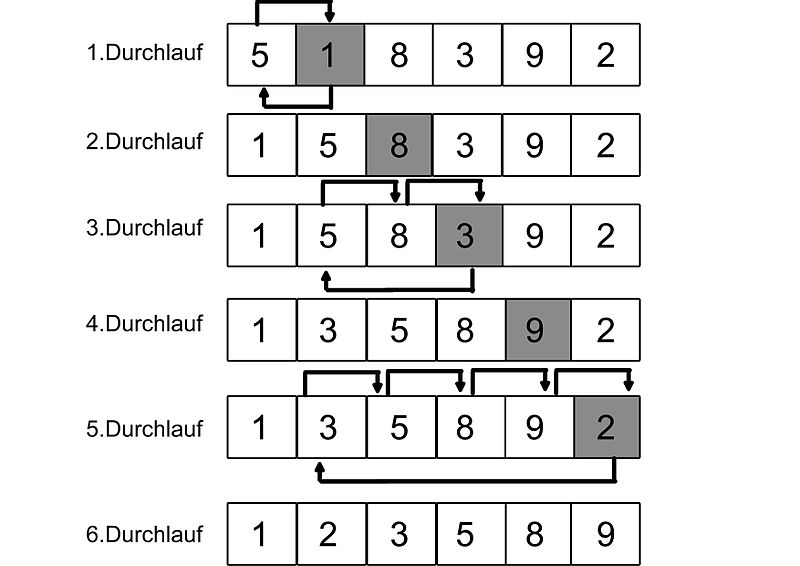
\includegraphics{InsertionSort}
\end{frame}

\subsection{Quicksort}
\begin{frame}[fragile]{Quicksort}

\end{frame}

\subsection{Bucketsort}


\end{frame}

\end{document}
